\documentclass[tikz,border=0pt]{standalone}
\usepackage{xcolor}
\definecolor{timblue}{RGB}{0,0,255}
\begin{document}
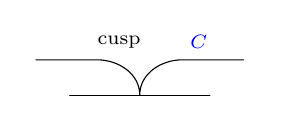
\begin{tikzpicture}[x=1pt,y=-1pt,line width=0.3985pt,line cap=round,line join=round]
  \path[use as bounding box] (0,0) rectangle (81.485,27.237);

  % Exact transcription of the accepted VII SVG path.
  \draw
    (2.992187,11.612690) --
    (25.117187,11.612690)
    .. controls (32.617187,11.612690) and (40.492187,16.488281) ..
    (40.492187,24.363282)
    .. controls (40.492187,16.488281) and (48.367188,11.612690) ..
    (55.867187,11.612690) --
    (77.992188,11.612690);

  \draw (15.179687,24.363282) -- (65.804688,24.363282);

  \node[anchor=base west,inner sep=0pt,font=\fontsize{7}{8}\selectfont]
    at (25.079280,6.223655) {cusp};
  \node[anchor=base west,inner sep=0pt,text=timblue,font=\fontsize{7}{8}\selectfont]
    at (58.474760,7.542704) {$C$};
\end{tikzpicture}
\end{document}
